\documentclass[11pt]{article}
\usepackage{geometry}                
\geometry{letterpaper}                 
\usepackage[parfill]{parskip}        
\usepackage{graphicx}
\usepackage{amssymb}
\usepackage{amsmath}
\usepackage{courier}
\usepackage{epstopdf}
\usepackage{verbatim}
\usepackage{float}
\usepackage{enumerate}
\usepackage{hyperref}
\usepackage[utf8]{inputenc}
\usepackage[T1]{fontenc}
\DeclareGraphicsRule{.tif}{png}{.png}{`convert #1 `dirname #1`/`basename #1 .tif`.png}
\usepackage{color}
\usepackage{textcomp}
\definecolor{listinggray}{gray}{0.9}
\definecolor{lbcolor}{rgb}{1,1,1}

\begin{document}
{\small
\section*{Problems for Discussion 8, 11/12/13}
Compiled by Mai Le
}

\section{DFT properties}
% Fessler exam 3 of Winter 2004, number 6
Determine the output of the following Matlab command: 

\texttt{fft(fft([3 4 5 6]))}

% and number 7
Determine the output of the following Matlab command:

\texttt{ifft(fft([1 2 3 0 0 0].*fft([1 0 1 0 0 0]))}

\section{Rational Rate Conversion}
% Fessler exam 3 of Winder 2004, number 8 and 9
A signal $x_a(t)$ was sampled at rate $F_1 = 30$ kHz and its samples $x_1[n]$ were stored. Later it is decided to recover this signal using an D/A converter that works at the sampling rate $F_2 = 20$ kHz. The following system has been proposed for solving this sampling rate conversion problem.

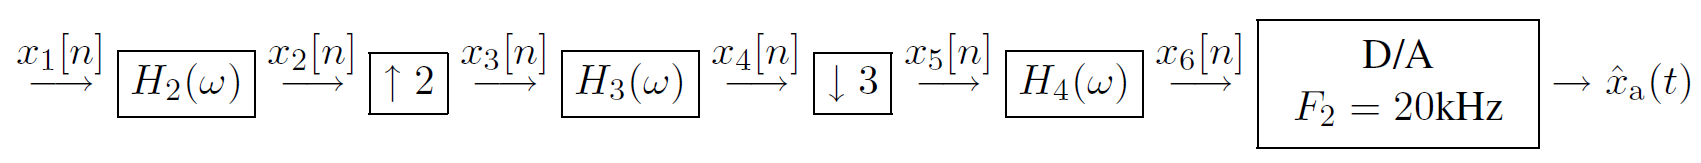
\includegraphics[width = 0.9\textwidth]{rate_conv_a.png} 

\begin{description}
	\item[(a)] Specify the magnitude responses of the three filters $H_2(\omega)$, $H_3(\omega)$, $H_4(\omega)$ so that the final output signal will be as close to the original signal as possible. If a filter is not needed, say so.
	\item[(b)] The following alternative system for solving the preceding rate conversion problem has also been proposed. Explain why this system would be (1) preferable, (2) inferior, or (3) equivalent to the system proposed in part (a).
	
	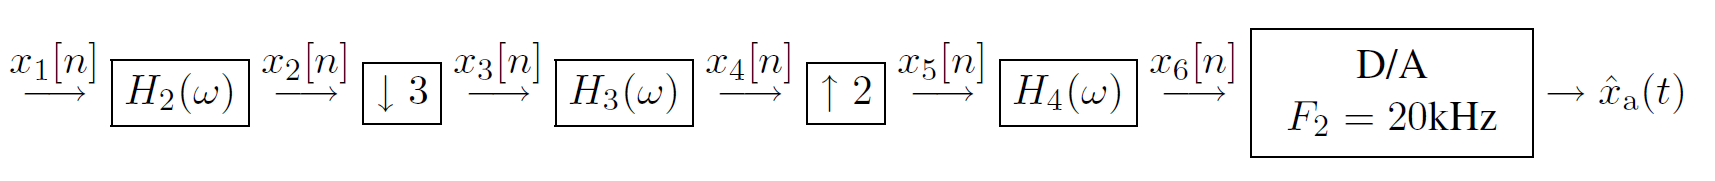
\includegraphics[width = 0.9\textwidth]{rate_conv_b.png} 	
\end{description}

\section{DFT lengths}
% Fessler exam 3, Fall 1998, problem 1b

Suppose $x[n]$ is time-limited to $n=0,1, 2, 3$ and the 8-point DFT of $x[n]$ is given by

\[ \{\underline{5}, 3-j\sqrt{2}, 3, 3-j\sqrt{2}, 1, 3+j\sqrt{2}, 3, 3+j\sqrt{2} \} \]

Find the 4-point DFT of $x[n]$.

\section{DFT from the DTFT}
% Fessler exam 3, Fall 1998, problem 2a

A signal $x[n]$ has DTFT $X(\omega) = 4e^{-j13 \omega} + 3e^{j2\omega} + 2e^{-j11\omega}+7$. Find the 11-point inverse DFT of $\{X(\omega)\big|_{\omega = 2 \pi k /11}, k = 0,\ldots, 10\}$.

\section{Uncertainty Principle}

For a signal $x[n]$ and its N-point DFT $X[k]$, 

\[ |support(x)||support(X)| \leq N \]

where the support of a signal is defined as:

\[ support(x)=\{n, x[n] \neq 0\},\ |support(x)| = \text{ number of elements in } support(x) \]



\end{document}